%%%%%%%%%%%%%%%%%%%%%%%% An example chapter %%%%%%%%%%%%%%%%%%%%%%%%%%%%%%%%%%%%%%%%%%%
%[Chapter name as it will appear in the ToC]{chapter name as it will apear as the title to the chapter} - you probably always want them to be the same, but you might not, so use case demonstrated here
\chapter[High ice-nucleating particle concentrations associated with Arctic haze in springtime cold-air outbreaks]{High ice-nucleating particle concentrations associated with Arctic haze in springtime cold-air outbreaks}
\label{ch:measurements}
% shorter title for your header
\chaptermark{High INP concentrations associated with Arctic Haze in spring CAOs} 
%%%%%%%%%%%%%%%%%%%%%%%% Example of content %%%%%%%%%%%%%%%%%%%%%%%%%%%%%%%%%%%%%%%%%%%
% Note the use of:
% Cross-referencing using \cref that automatically gives "Figure 1".
% Use of \citep and and \citet to cite papers in parentheses and inline respectively.
% Use of \qty and \qtyrange to correctly use SI units and format quantities.
% Use of a sideways table
% Use of a tabularx table
% Use of equation and align environments.
% Headers in practice.
% Clear double page doesn't produce a blank page at the end this time as the final page
% is even-numbered.
% Inclusion of figure. Using the wrapfig environment, it is possible to push this to
% one side of the page and wrap text around it instead. To be honest, I would not
% recommend this for the sake of your examiners, especially as justified text around a
% figure often looks nasty.
% I have chosen not to use the subfigure facility and to make each figure a standalone
% as this is what journals often need anyway.
\section*{Abstract}
A section for the abstract that deliberately does not appear in the ToC.
Work in this excerpt was taken from Raif, E. N., Barr, S. L., Tarn, M. D., McQuaid, J. B., Daily, M. I., Abel, S. J., Barrett, P. A., Bower, K. N., Field, P. R., Carslaw, K. S., and Murray, B. J.: High ice-nucleating particle concentrations associated with Arctic haze in springtime cold-air outbreaks, Atmos. Chem. Phys., 24, 14045–14072, https://doi.org/10.5194/acp-24-14045-2024, 2024.

\section{Excerpt from paper}

\cref{fig:cao}a shows the potential sources of INPs for CAO clouds in the Northern Hemisphere.
Potential Arctic sources of INPs are biogenic material from sea-spray \citep{wilson_marine_2015, demott_sea_2016, mccluskey_marine_2018} and terrestrial INPs from high-latitude sources \citep{kawai_dominant_2023}.
Potential terrestrial sources of INPs include glacial outwash sediments \citep{tobo_glacially_2019, xi_ice_2022, barr_southern_2023}, sandy deserts in Iceland \citep{sanchez-marroquin_iceland_2020}, boreal forests \citep{brasseur_measurement_2022}, Arctic surface vegetation \citep{pereira_freitas_regionally_2023} and thawing permafrost \citep{creamean_thawing_2020}.
In addition, Arctic aerosol can have lifetimes of many weeks, which results in the build up of Arctic haze in winter and spring \citep{stohl_characteristics_2006}.
Accordingly, it is also possible that INPs entering CAOs may have been transported into the Arctic from lower latitudes where they reside in the stable Arctic atmosphere before being transported out again in CAOs \citep{carslaw_chapter_2022}.
Different types of INPs have different characteristic ranges of freezing temperatures \citep{kanji_overview_2017}.
This means understanding the aerosol sources that contribute to the INP population in CAO clouds can reduce the uncertainty in the cloud-phase feedback.

Aerosol concentrations near the sea surface ($<\qty{500}{\meter}\text{~a.s.l.}$) were consistently \qtyrange{100}{200}{\per\centi\meter\cubed}.

\begin{figure}[t]
    \centering
    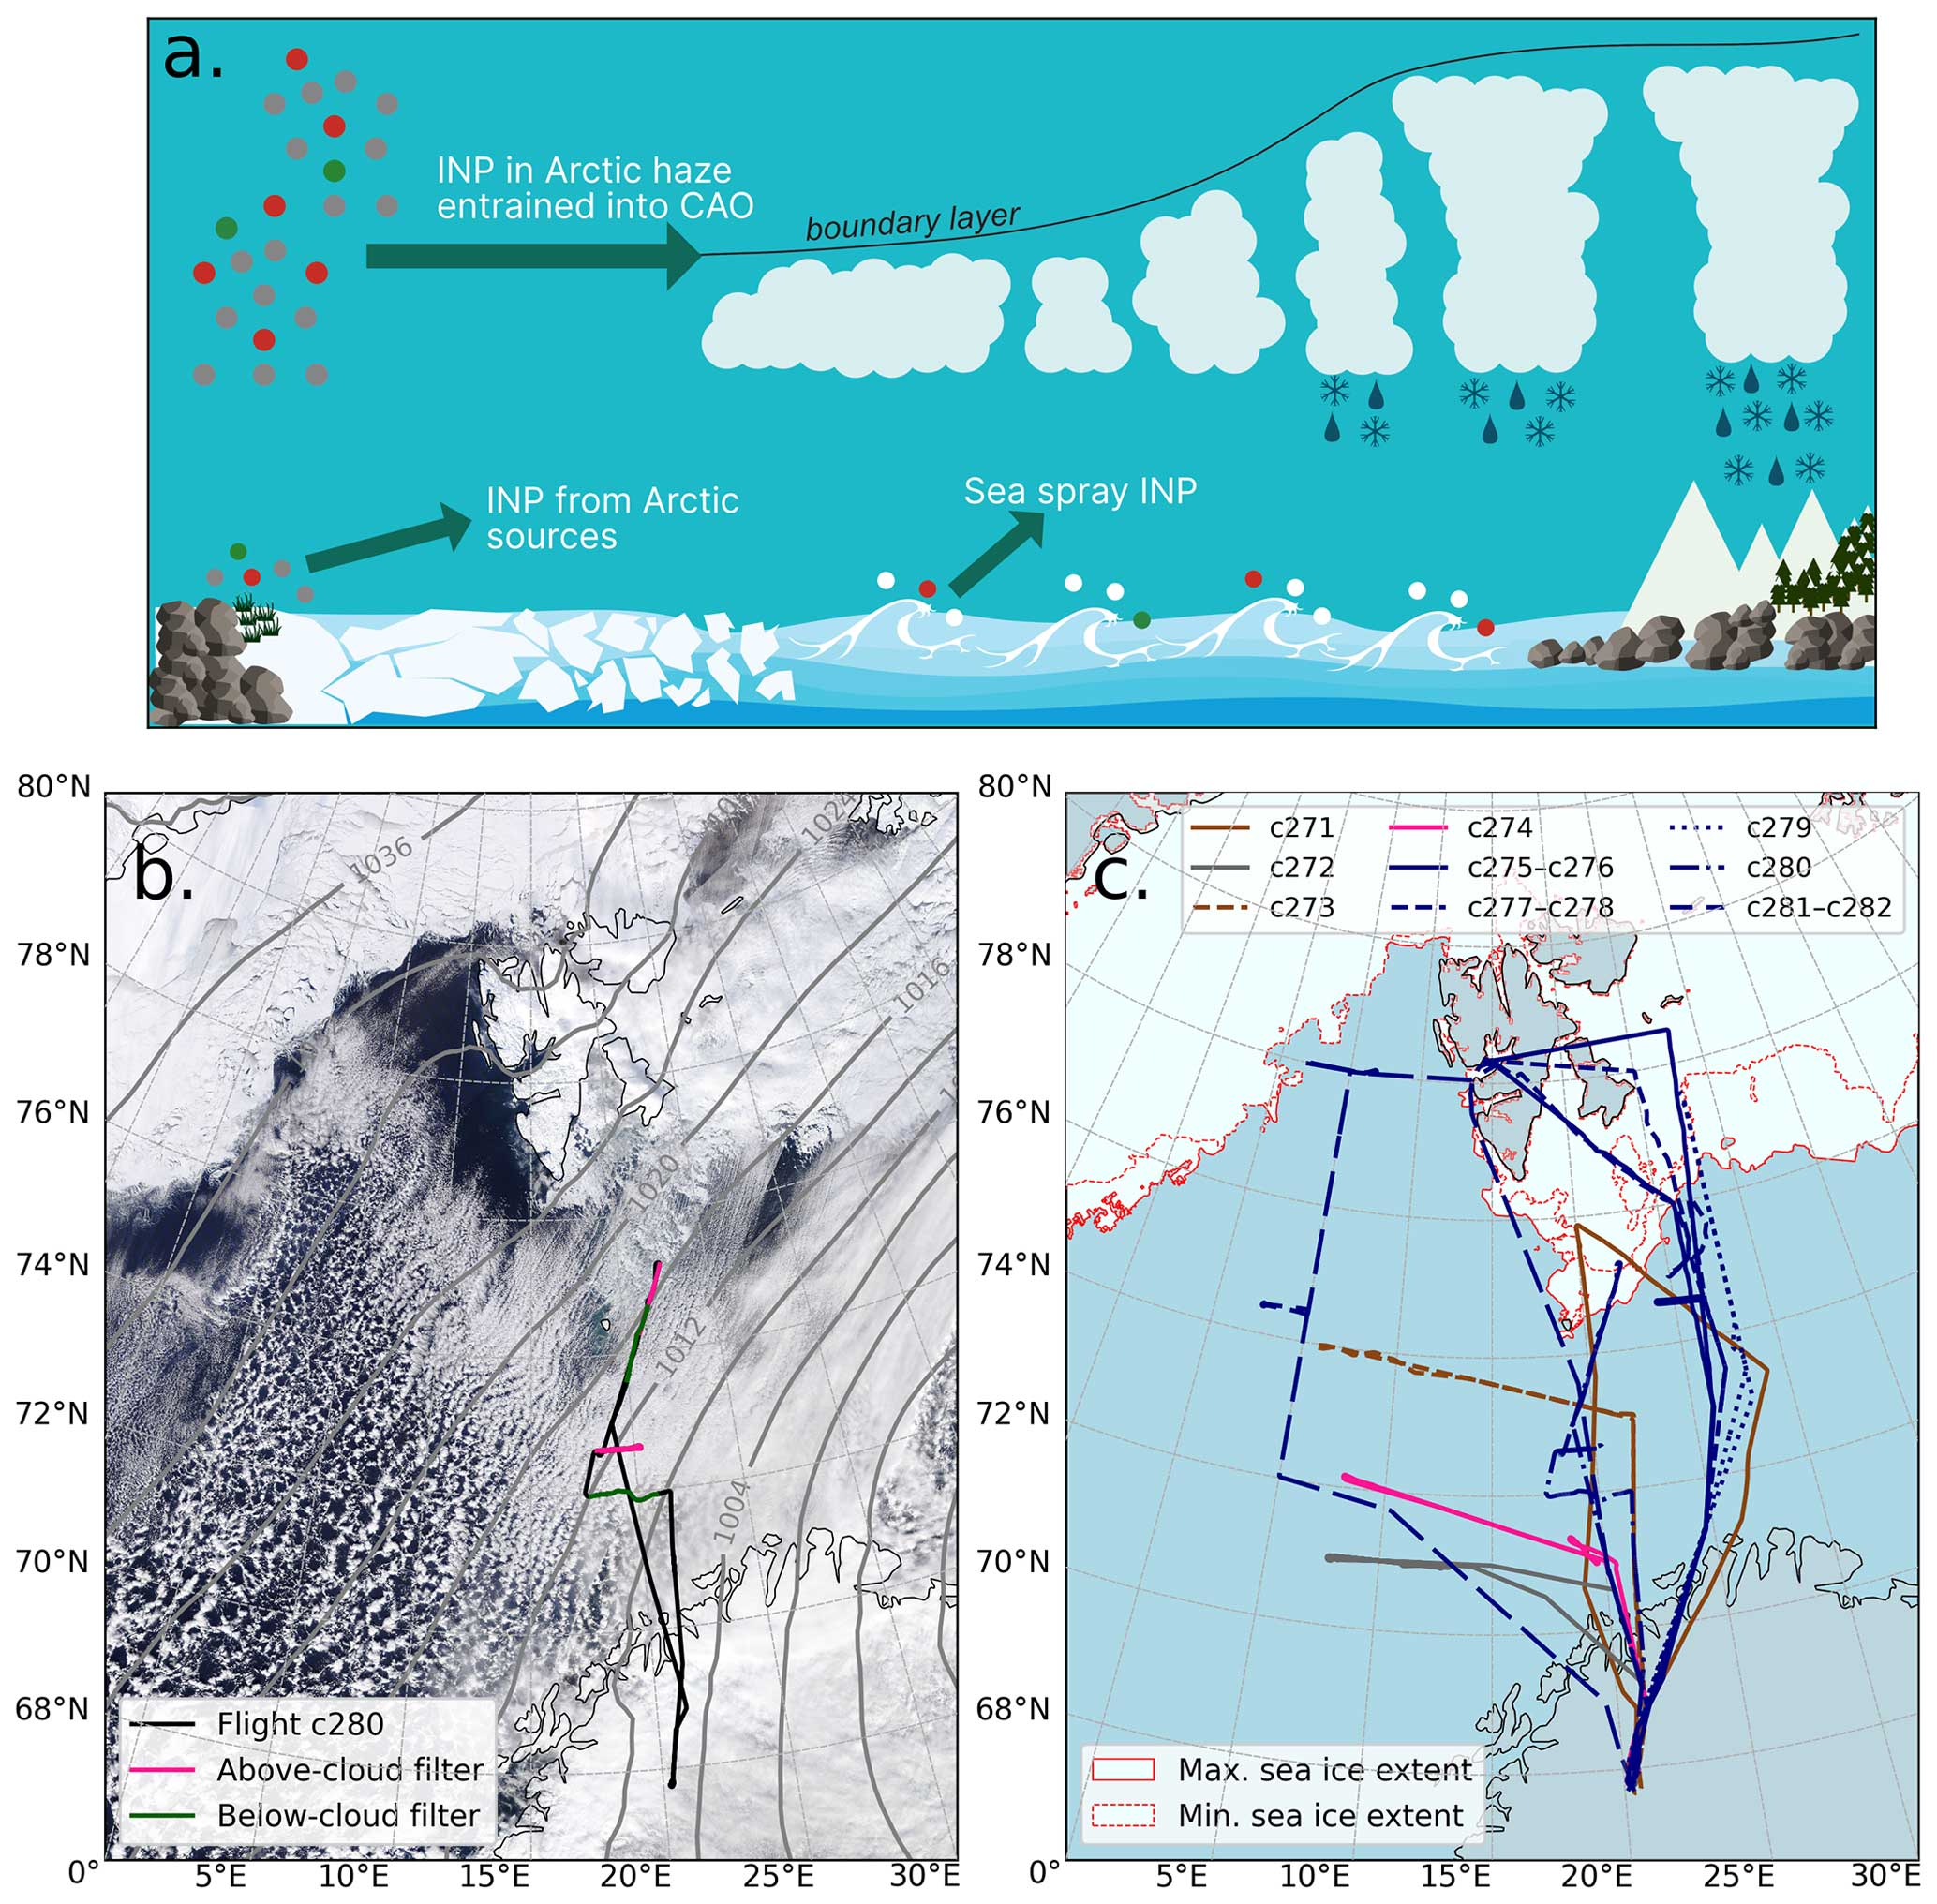
\includegraphics[width=\linewidth]{images/paper_figs/paper_f01.jpg}
    \caption[CAO schematic with an example of an ACAO flight (c280) overlaid on a satellite image and all flight paths during the ACAO]{For brevity, the full caption is excluded but thanks to MODIS, the US National Ice Center (MASIE) and ECMWF (ERA5) and the Facility for Airborne Atmospheric Measurements for data used in these plots.} 
    \label{fig:cao}
\end{figure}


\subsection{Results}

These sampling locations were considered to represent air below, above and before the development of the atmospheric boundary layer over sea respectively.
The locations, altitudes and purpose of each filter measurement are shown in \cref{tab:filter_table}.

\begin{sidewaystable}[p]
    \caption{Times, locations and sampling intent of all filter samples made during the campaign.}
    \begin{tabular}{llcccrrrll}
    \hline\hline
    {Sample ID} &
    {Run type} &
    \begin{tabular}[t]{@{}c@{}}Date\\ (mm-dd)\end{tabular} &
    {Start (UTC)} &
    {End (UTC)} &
    \begin{tabular}[t]{@{}l@{}}Mean\\ alt. \unit{\metre}\end{tabular} &
    \begin{tabular}[t]{@{}l@{}}Mean\\ lat. (\degree~N)\end{tabular} &
    \begin{tabular}[t]{@{}l@{}}Mean\\ lon.(\degree~E)\end{tabular} &
    \begin{tabular}[t]{@{}l@{}}CAO\\ flow\end{tabular} &
    {Notes} \\
    \hline\hline
    {c271r1} & above cloud & 03-11 & 09:40:07 & 10:07:24 & 1747 & 74.3 & 20.3 & W & ~ \\
    \hline
    {c271r2} & below cloud & 03-11 & 10:18:03 & 10:42:48 & 39 & 75.5 & 21.5 & W & \qty{2}{\minute} pause during aircraft turning\\
    \hline
    {c271r3} & below cloud & 03-11 & 11:18:05 & 11:38:38 & 49 & 72.7 & 27.9 & W & filter processed \qty{3}{\day} after collection \\
    &&&&&&&&&two pauses for precipitation\\
    \hline
    {c272r6} & above cloud & 03-16 & 12:07:25 & 12:34:15 & 2957 & 71.0 & 10.5 & N/A & warm-air intrusion conditions\\
    \hline
    {c273r1} & above cloud & 03-19 & 12:01:25 & 12:38:51 & 3403 & 73.8 & 11.2 & W & ~  \\
    \hline
    {c273r2} & below cloud & 03-19 & 12:54:07 & 13:13:35 & 415 & 73.9 & 8.7 & W & two short pauses to avoid showers  \\
    \hline
    {c274r1} & above cloud & 03-21 & 13:47:10 & 14:07:23 & 2672 & 71.8 & 12.6 & NW & ~  \\
    \hline
    {c274r3} & below cloud & 03-21 & 15:18:08 & 15:41:22 & 165 & 71.2 & 19.3 & NW & two short pauses for aircraft turning\\
    &&&&&&&&&and one pause to avoid showers\\
    \hline
    {c275r1} & below cloud & 03-23 & 10:03:37 & 10:28:22 & 162 & 76.5 & 23.8 & N & ~  \\
    \hline
    {c276r2} & upstream & 03-23 & 12:55:29 & 13:20:29 & 1711 & 78.5 & 22.0 & N & ~  \\
    \hline
    {c276r4} & below cloud & 03-23 & 14:32:27 & 14:55:27 & 156 & 74.6 & 25.2 & N & ~  \\
    \hline
    {c277r1} & below cloud & 03-24 & 10:30:52 & 10:59:06 & 159 & 76.7 & 22.8 & N & two pauses for altitude increases \\
    &&&&&&&&&cloud in very early stages of formation \\
    \hline
    {c278r2} & upstream & 03-24 & 13:02:05 & 13:26:16 & 1725 & 78.2 & 21.3 & N & ~  \\
    \hline
    {c278r4} & below cloud & 03-24 & 14:07:00 & 14:31:56 & 333 & 75.1 & 26.0 & N & \qty{2}{\minute} pause for turning due to precip. \\
    \hline
    {c279r1} & below cloud & 03-25 & 11:23:21 & 11:44:12 & 155 & 76.9 & 28.0 & N & ~  \\
    \hline
    {c279r2} & above cloud & 03-25 & 11:48:26 & 12:08:44 & 1323 & 75.4 & 28.0 & N & ~  \\
    \hline
    {c280r1} & above cloud & 03-29 & 09:29:00 & 09:49:17 & 1573 & 74.8 & 21.6 & N & ~  \\
    \hline
    {c280r2} & below cloud & 03-29 & 09:59:55 & 10:15:58 & 327 & 74.1 & 20.6 & N & ~  \\
    \hline
    {c280r3} & above cloud & 03-29 & 10:34:01 & 10:54:06 & 2013 & 72.6 & 19.4 & N & 2\,min pause during aircraft turning\\
    \hline
    {c280r4} & below cloud & 03-29 & 11:05:35 & 11:24:51 & 334 & 72.0 & 19.3 & N & 1\,min pause to avoid showers \\
    \hline
    {c282r1} & above cloud & 03-30 & 12:08:32 & 12:28:27 & 1761 & 78.0 & 7.5 & N & ~  \\
    \hline
    {c282r3} & below cloud & 03-30 & 14:02:12  & 14:26:08 & 307 & 74.4 & 3.5 & N & \qty{4}{\minute} pause during aircraft turning  \\
    \hline\hline
    \end{tabular}
   \label{tab:filter_table}
\end{sidewaystable}


\begin{equation}
    \label{eq:median_INP}
    \overline{N}_\mathrm{INP} = \overline{a} \exp{\left[\overline{b}\left(\overline{c}-T\right)^{\overline{d}}\right]},
\end{equation}



\begin{table}[t]
\begin{tabularx}{\linewidth}{llLllll}
\hline
\hline
Flight & Upwind filter & Downwind filter & $\Delta\varphi$ &
$F_{\mathrm{INP}}$  &
$F_{\mathrm{S}}$   &
$F_{\mathrm{aer}}$  \\
\hline \hline
c275--276 & c275r1, Sc & c276r4t, Sc & 1.92 & 0.40 & 0.52 & 0.75 \\ \hline
c280   & c280r2, Sc & c280r4t, precipitating Cu & 2.17 & 0.35 & 0.19 & 1.85 \\ \hline
c281-282 & c282r2, Sc  & c282r3t, precipitating Sc--Cu & 3.58 & 0.68 & 0.39 & 1.69 \\
\hline
\hline
\end{tabularx}
\label{tab:up_and_down}
\caption[Factors of change in INP and aerosol properties between pairs of below-cloud samples]{Factors of change in the INP concentration at \qty{-15}{\degreeCelsius} ($F_{\mathrm{INP}}$), INP concentration normalised by surface area at \qty{-15}{\degreeCelsius} ($F_{\mathrm{S}}$) and total aerosol surface area ($F_{\mathrm{aer}}$) between three pairs of below-cloud filter measurements.}
\end{table}

Using the values of $N_\mathrm{INP}(\qty{-15}{\degreeCelsius})$ and the total aerosol surface area $S_\mathrm{aer}$, we calculated the factors of change in INP concentration ($F_{\mathrm{INP}}$), ice-nucleating activity ($F_{\mathrm{S}}$) and surface area ($F_\mathrm{aer}$) between the upwind and downwind measurements:
\begin{align}
F_{\mathrm{INP}} &= \frac{{N_{\mathrm{INP}}\left(\qty{-15}{\degreeCelsius},\:\mathrm{downwind}\right)}}{{N_{\mathrm{INP}}\left(\qty{-15}{\degreeCelsius},\:\mathrm{upwind}\right)}},\\
F_{\mathrm{S}} &= \frac{{N_{\mathrm{INP}}\left(\qty{-15}{\degreeCelsius},\:\mathrm{downwind}\right)}/S_{\mathrm{aer}}~(\mathrm{downwind})}{{N_{\mathrm{INP}}\left(\qty{-15}{\degreeCelsius},\:\mathrm{upwind}\right)}/S_{\mathrm{aer}}~(\mathrm{upwind})},\\
F_{\mathrm{aer}} &= \frac{S_{\mathrm{aer}}\left(\mathrm{downwind}\right)}{S_{\mathrm{aer}}\left(\mathrm{upwind}\right)}.
\end{align}
These values are displayed in \cref{tab:up_and_down} with the difference in latitude between the measurements, $\Delta\varphi$.
Both the INP concentration and the ice-nucleating activity decreased with latitude.
The total surface area of the aerosol increased in two flights by \qty{69}{\percent} and \qty{85}{\percent} but decreased by \qty{25}{\percent} in one pair.
The upwind filters were sampled under stratocumulus conditions, while the downwind filters were in a mixture of stratocumulus and cumulus, with precipitation in two cases (c280r4 and c282r3).

